\section{Results}
\label{sec:results}

Table~\ref{tab:did} reports every estimate of~\eqref{eq:did}; Figure~\ref{fig:claims} plots the three headline coefficients side by side for the two eras. The short version: the AI era looks nothing like the IT boom in the labor data, and the difference points to substitution.

\begin{table}[t]
\caption{Difference-in-differences estimates of~\eqref{eq:did}. Each coefficient is the change in the outcome during the era, relative to baseline, for a sector one standard deviation more exposed. Standard errors are clustered by sector; $p_{\text{boot}}$ is from the wild cluster bootstrap (Webb weights, 1,999 replications). C1 and C3: 13 sectors, annual. C2: 19 sectors, quarterly.}
\label{tab:did}
\inserttable{tab_did}
\end{table}

\begin{figure}[t]
  \centering
  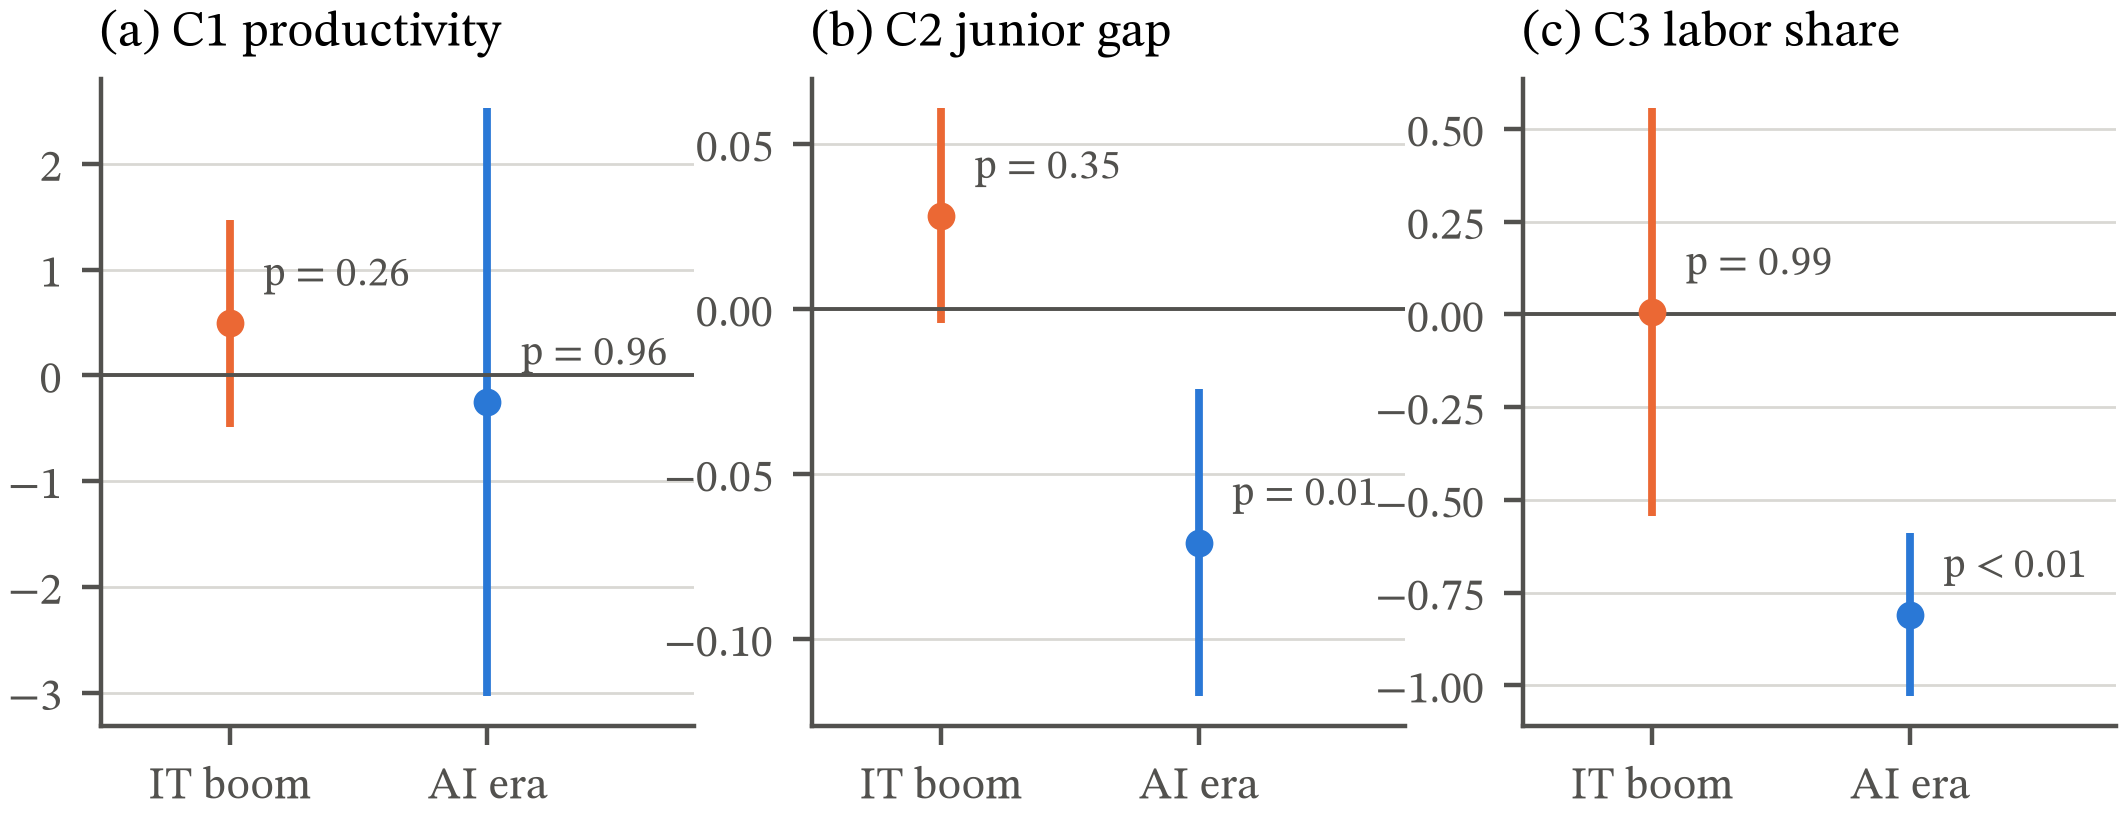
\includegraphics[width=\textwidth]{fig03_claims_it_vs_ai.png}
  \caption{IT boom versus AI era. Coefficients from Table~\ref{tab:did} with 95\% intervals and bootstrap $p$-values: (a) output per hour growth, pp per year; (b) junior employment gap given sector size, log points; (c) change in the labor share, pp per year. Orange: IT boom, exposure is the 1995 IT capital share. Blue: AI era, exposure is language-model AI exposure.}
  \label{fig:claims}
\end{figure}

\subsection{C1: no productivity acceleration yet}

Output per hour did not accelerate faster in AI-exposed sectors. The AI-era coefficient is $-0.26$ percentage points per year per standard deviation, with a standard error of 1.42 and a bootstrap $p$ of 0.96. In the IT boom the estimate is $+0.49$, positive as \citet{stiroh2002it} found but imprecise with 13 sectors ($p=0.26$). We read the AI-era null with care. It is a statement about measured output: when a firm buys an AI service, the purchase is an intermediate input and is subtracted from the firm's value added (Assignment~1, Question~1). A firm that uses AI to replace a junior analyst may produce the same output with fewer hours, which raises output per hour, or the same hours with a higher bill for purchased services, which does not. Measured productivity in the user industry then understates the gain, which is consistent with the J-curve argument of \citet{brynjolfsson2021jcurve}. Our earlier descriptive table, which suggested a white-collar productivity surge, did not survive the switch to all-employee hours and the inclusion of time effects; we discarded it.

\subsection{C2: the missing juniors}

The clearest result is in employment by age. In the AI era, a sector one standard deviation more exposed saw the employment of 22--24 year-olds fall by 4.9 log points relative to 35--54 year-olds in the same sector; holding sector size fixed the decline is 7.1 log points (bootstrap $p=0.01$). The hiring gap moves in the same direction ($-3.3$ and $-4.6$ log points), consistent with adjustment through hiring rather than separations, as \citet{brynjolfsson2025canaries} find in ADP microdata. In the IT boom the sign is reversed (+3.2 and +2.8 log points) though not significant: computers complemented young, computer-literate workers.

\begin{figure}[t]
  \centering
  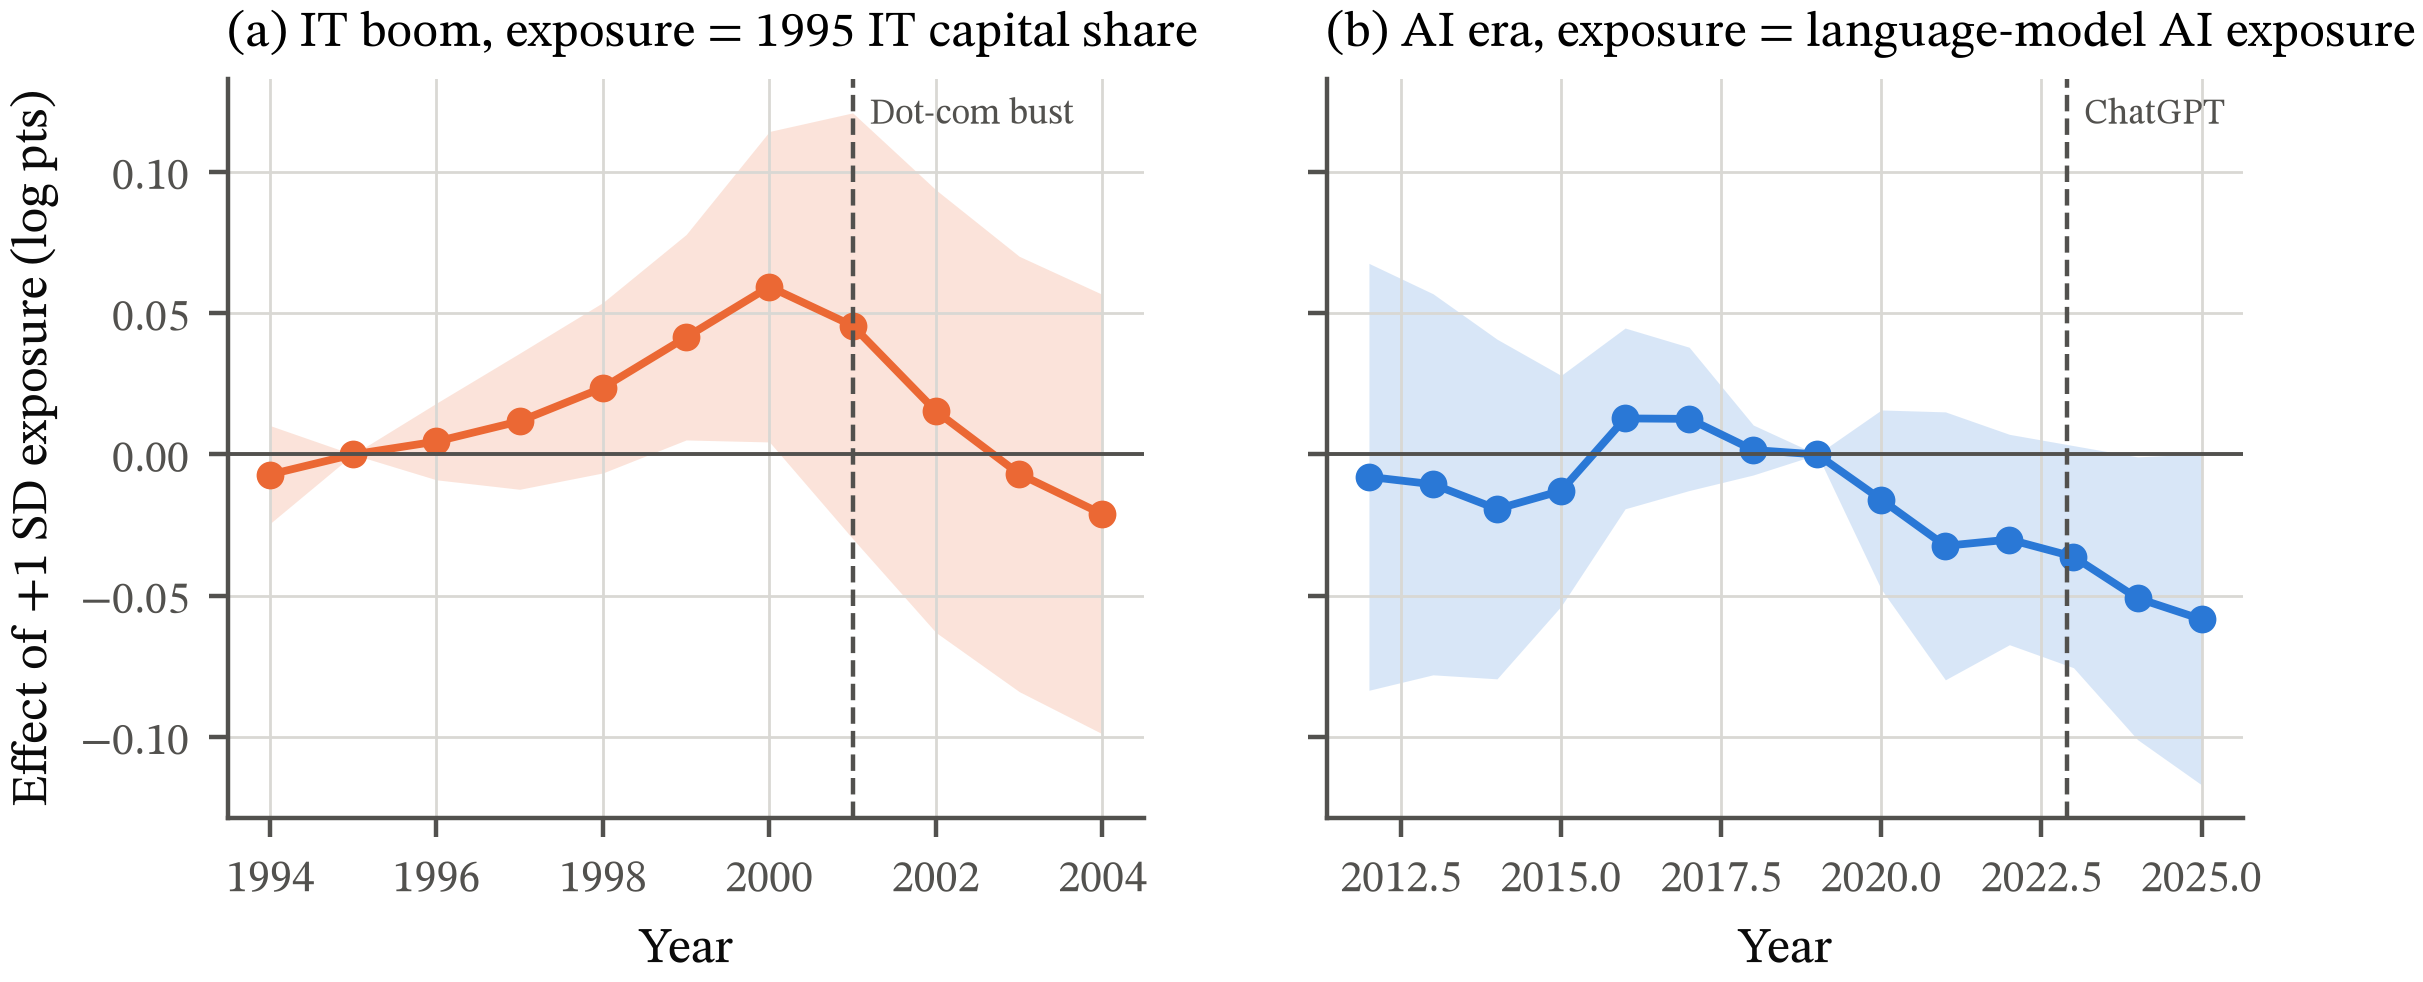
\includegraphics[width=\textwidth]{fig02_c2_event_studies.png}
  \caption{Event studies of the junior employment gap. Each point is the effect of one standard deviation of exposure on the junior gap in that year, relative to the base year (1995 for the IT boom, 2019 for the AI era), with 95\% intervals. (a) IT boom; the dashed line marks the 2001 dot-com bust. (b) AI era; the dashed line marks ChatGPT's release.}
  \label{fig:eventstudy}
\end{figure}

Timing matters for attribution, and Figure~\ref{fig:eventstudy} shows it. Panel (b) is flat from 2012 to 2019, so exposed sectors were not already shedding juniors. The decline starts in 2020, before ChatGPT, and continues through 2025. Panel (a) is a useful warning: in the IT boom, juniors in IT-intensive sectors gained through 2000 and lost those gains in the dot-com bust. Junior employment is cyclical; a hiring freeze in rate-sensitive sectors can look like technology.

\begin{table}[t]
\caption{Did the trend bend at ChatGPT? Each row is a term interacted with standardized AI exposure; COVID years (2020--2021) are dropped. The junior gap regression controls for sector size. Bootstrap $p$-values as in Table~\ref{tab:did}.}
\label{tab:kink}
\inserttable{tab_kink}
\end{table}

Table~\ref{tab:kink} separates the two stories. With COVID years dropped, exposed sectors show no pre-existing trend (0.0002 per year), a post-COVID level drop of 5.6 log points ($p<0.01$), and an \emph{additional} decline of 1.2 log points per year after ChatGPT ($p=0.01$). The level shift is consistent with remote work and the 2022 hiring freeze; the post-ChatGPT slope is what a substitution story predicts. This conclusion depends on how the COVID years are handled: an earlier specification that fitted a straight line through 2020--2022 averaged the crash and recovery into a single slope and found no post-ChatGPT kink. We report both, and treat the kink as suggestive rather than settled.

Total employment tells a different story from employment by age. Across 91 detailed CES industries, AI exposure predicts no change in total employment: no level shift, no kink (Table~\ref{tab:kink}, right columns; Figure~\ref{fig:detailed} in the appendix). AI is not, so far, reducing headcount in exposed industries; it is changing who is hired.

\subsection{C3: who gets paid}

The labor share answers the incidence question. In the AI era, a sector one standard deviation more exposed saw its labor share fall by 0.81 percentage points per year relative to baseline (bootstrap $p<0.01$); in the IT boom the estimate is zero (0.006, $p=0.99$). Because finance has by far the highest exposure, and its margins rose with interest rates in 2023--24 for reasons unrelated to AI, we re-estimate the model dropping one sector at a time. The coefficient stays between $-0.61$ (without finance) and $-0.85$, and every bootstrap $p$ stays below 0.01. Value-added prices in exposed sectors did not fall relative to others (+2.2 pp per year, $p=0.26$), so the gain was not passed on to consumers.

\subsection{Reading the three together}

The pieces fit one story. AI-exposed sectors are hiring fewer juniors, are not shrinking overall, are not (yet) producing measurably more per hour, and are paying a smaller share of their value added to labor. That is substitution at the entry margin, with the gain accruing to capital: the routine tasks of junior staff are being done by purchased AI services and by the seniors who remain. The IT boom, by contrast, looked like complementarity. For an investor this is a cash-flow signal (margins in exposed sectors should be higher than their measured productivity suggests), which brings us to whether prices reflect it.

\subsection{Pooling the IT prior with AI-era evidence}
\label{sec:bayes}

How much should the IT boom inform our reading of AI? We treat the IT-era estimate as a prior for the AI-era coefficient, $\beta_{AI} \sim N(\hat\beta_{IT}, \mathrm{se}_{IT}^2 + \tau^2)$, where $\tau$ measures how different we allow AI to be, and update with the AI-era estimate. Figure~\ref{fig:bayes} traces the posterior as $\tau$ widens. For C3 the AI data dominate even at $\tau=0$: the posterior mean is $-0.70$, because the AI-era estimate is far more precise than the prior. For C2 the conclusion depends on beliefs: if AI is assumed identical to IT the posterior is centered near zero, but once $\tau$ reaches the AI-era standard error the probability that the effect is negative rises to 0.95. For C1 neither era is informative.

\begin{figure}[t]
  \centering
  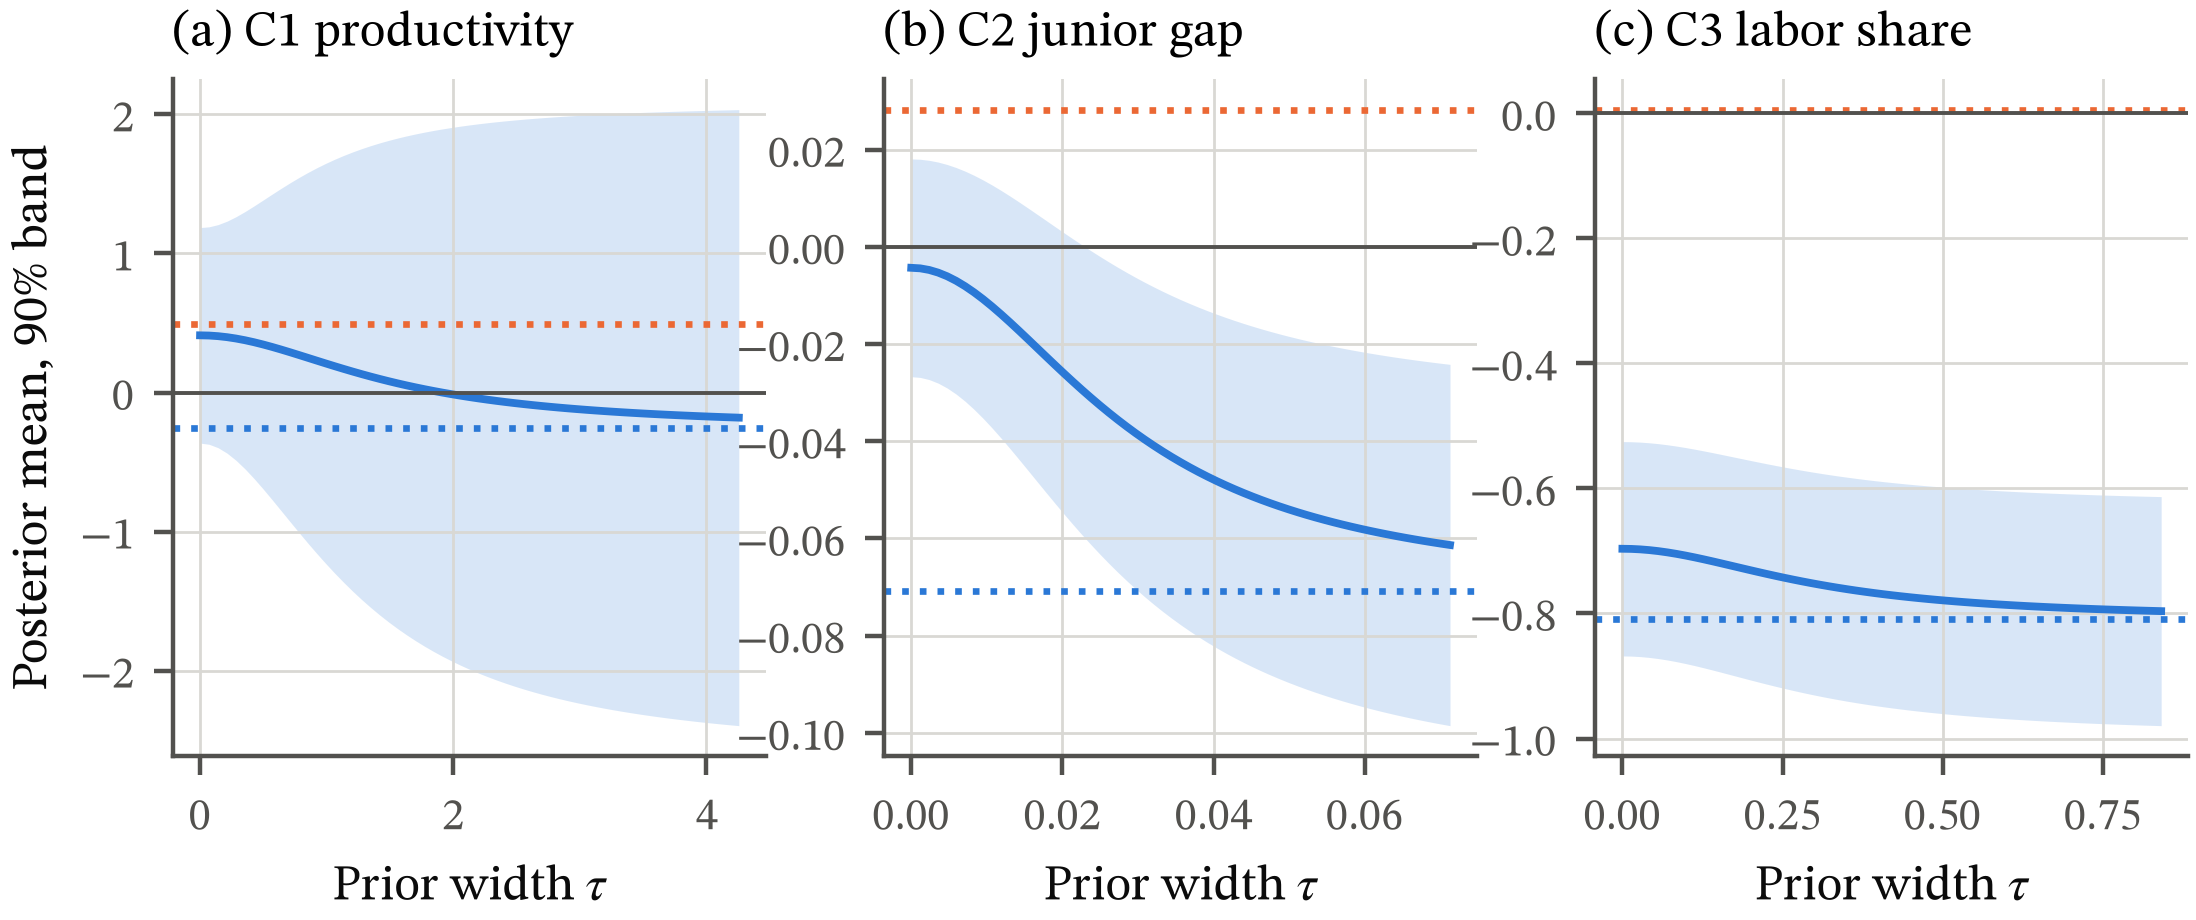
\includegraphics[width=\textwidth]{fig08_bayesian_pooling.png}
  \caption{Posterior of each AI-era coefficient when the IT-boom estimate is used as a prior, as the prior width $\tau$ increases from ``AI is exactly IT'' ($\tau=0$) to ``AI is new''. Solid line: posterior mean, with 90\% band. Dotted lines: the IT-era estimate (orange) and the AI-era estimate (blue).}
  \label{fig:bayes}
\end{figure}
